To validate the local-geometry-aware complementarity-based rigid-contact modeling strategy developed above, the experiments in this section are organized along the progression of ``basic correctness, extended correctness, continuous-contact capability, industrial-scale performance, remaining limitations, and computational efficiency.'' The first two head-on collision cases are used to verify the correctness of pure impulse transfer. This is followed by the eccentric disk--roller and Onset Stress benchmarks, which assess long-term adherence and contact-onset behavior in smooth continuous contact. An industrial cam benchmark is then used to evaluate accuracy and stability for complex engineering geometry. The Twin Gear case is used to expose the remaining limitations, and a final runtime comparison summarizes the evidence that, under regime-matched configurations, computational efficiency and contact-response accuracy can coexist. It should be stressed that these experiments do not aim to prove that one single regime or one single local representation is universally optimal across all benchmarks. Instead, each case is run under a preset regime matched to its contact state in order to assess the effectiveness and limitations of the proposed modeling strategy across different scenarios.

Unless otherwise stated, all compared methods are run in the same rigid-body dynamics environment and share the same time-stepping framework, external loading, output sampling, and benchmark-specific time-step settings. \texttt{Native Mesh} denotes the original mesh-based contact representation. \texttt{SdfFirstOrder} and \texttt{SdfSecondOrder} share the same SDF-based contact pipeline and differ only in the level of local geometric information used: the former uses only distance and first-order normal information, whereas the latter further introduces curvature feedforward. The direct difference between \texttt{SdfFirstOrder} and \texttt{SdfSecondOrder} therefore measures the incremental benefit of curvature feedforward, while the difference between mesh and the SDF path should be interpreted as an end-to-end comparison between the full local-geometry-aware modeling stack and the native contact representation. For continuous-sliding cases, the persistent manifold, local fitting, candidate filtering, and patch reduction together form the complete \texttt{SlidingPatch} path. The corresponding benchmarks therefore validate the effectiveness of the full modeling stack rather than the isolated effect of any single module.

Analytical references are used whenever available. When closed-form references are not available, external reference data independent of the present SDF pipeline are used instead. Specifically, the head-on collision and eccentric disk--roller cases use analytical references; the Onset Stress benchmark uses a piecewise analytical reference derived from the benchmark geometry and given kinematics; the industrial cam uses third-party reference curve data; and Twin Gear uses a commercial industrial software baseline. All runtimes are reported as end-to-end wall-clock time, so the broad phase, patch construction, and geometric-feedforward preprocessing in the SDF path are all included in the total runtime.

To ensure objective evaluation of computational cost and performance, all simulations were executed on the same high-performance workstation. The main hardware configuration consisted of an \textbf{AMD Ryzen 9 5900X 12-Core processor} and \textbf{16 GB of memory}. The software environment ran on Linux under Windows Subsystem for Linux 2 (WSL2). The code was compiled natively using GCC together with CMake, with a consistent highest-level optimization option such as \texttt{-O3} enabled globally.

\subsection{Basic correctness: head-on equal-sphere impact}
We first construct the most basic pure-impulse verification case: two spheres with identical radius and mass collide head-on along the same line. No gravity is applied, the friction coefficient is set to zero, and a translational joint constrains both bodies to a single translation direction so that lateral drift and attitude perturbations are excluded. The initial condition is set such that sphere A moves toward initially stationary sphere B with unit speed. Under perfectly elastic impact, the theoretical outcome is the classical one-dimensional velocity exchange: sphere A stops after impact and sphere B fully inherits the initial velocity of sphere A. Because the geometry, mass, and constraints are all analytically characterized, this case is appropriate as a basic physical-consistency test of the current shared SDF contact path in a pure-impulse setting rather than as an engineering-efficiency benchmark.

\begin{figure}[!t]
    \centering
    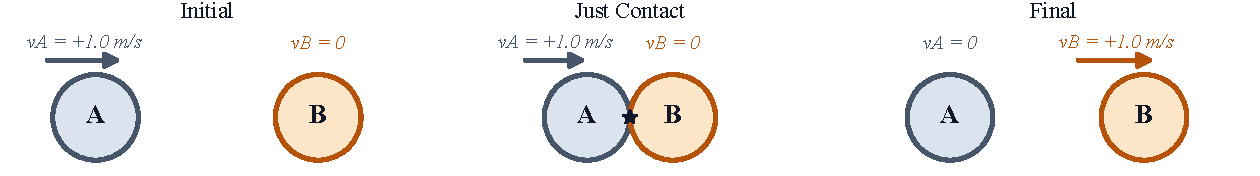
\includegraphics[width=\linewidth]{headon_equal_spheres_states.pdf}
    \caption{Three-stage model illustration of the equal-mass head-on collision case. From left to right: initial state, first contact, and final post-impact state. Velocity arrows indicate the direction and magnitude of the sphere velocities at each stage}
    \label{fig:headon_spheres_states}
\end{figure}

Figure \ref{fig:headon_spheres} shows the velocity histories of spheres A and B. On the current shared SDF contact path, both first-order and second-order SDF recover the ideal velocity exchange exactly in the discrete output: near the impact time, the velocity of sphere A jumps from $1.0$ m/s to $0.0$ m/s, while sphere B jumps from $0.0$ m/s to $1.0$ m/s. Their velocity RMSE relative to the analytical piecewise reference is therefore zero at the sampled output points.

By contrast, the native sphere contact still produces the correct final velocity exchange under the same time step, but exhibits a one-time-step switching delay in the discrete output, resulting in a velocity RMSE of $3.16\times10^{-2}$ m/s. This delay should be interpreted as a switching-time bias under the shared discrete step size rather than as an incorrect final impulse transfer. The result shows that the current SDF-based local-geometry-aware contact path can not only handle continuous sliding contact, but can also deliver correct momentum transfer in the most basic frictionless pure-impact setting, thereby establishing the physical-consistency foundation required for more general transient impact problems.

\begin{figure}[!t]
    \centering
    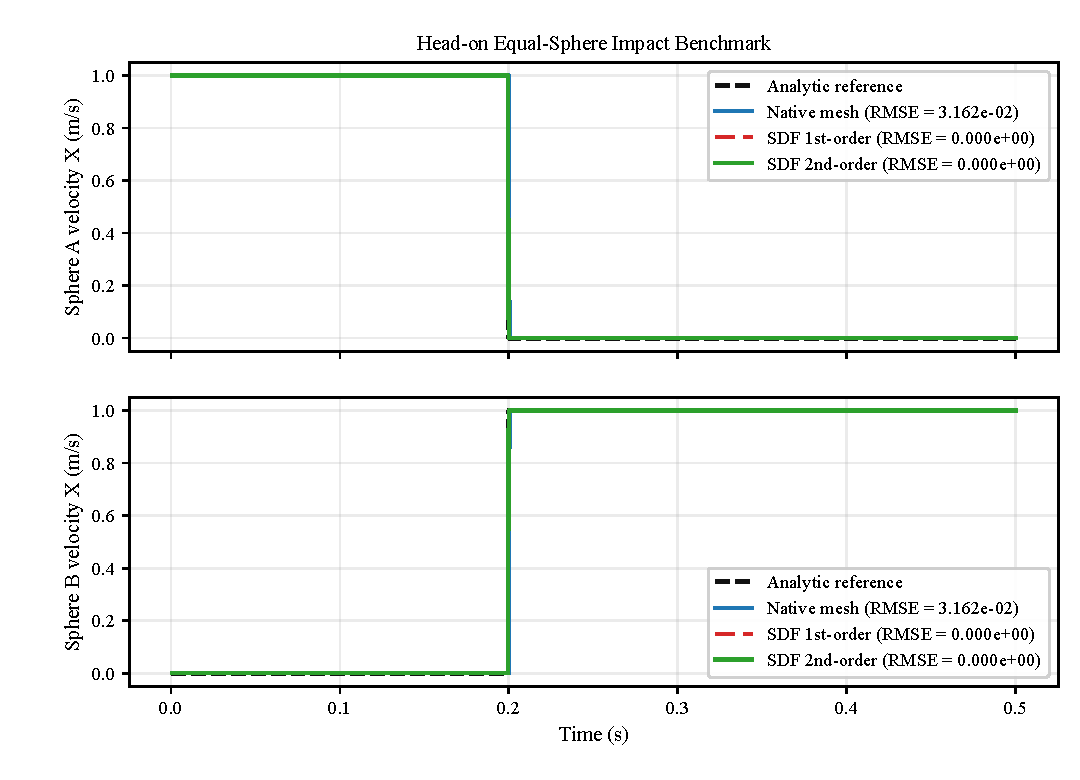
\includegraphics[width=0.94\linewidth]{headon_spheres_benchmark.pdf}
    \caption{Velocity histories for the equal-radius elastic head-on impact benchmark. Upper: sphere A. Lower: sphere B. The dashed black line denotes the analytical solution. Both SDF variants recover the ideal exchange, whereas the native mesh shows a switching lag of one time-step order}
    \label{fig:headon_spheres}
\end{figure}

\subsection{Extended correctness: head-on unequal-mass sphere impact}
To further confirm that the preceding conclusion is not limited to the special case of equal-mass velocity exchange, we construct an additional pure-impulse impact benchmark with equal radii but unequal masses. The two spheres keep the same radius, but sphere B is assigned twice the mass of sphere A. The initial condition is chosen such that sphere A is stationary and sphere B moves toward it along the constrained direction with velocity $-1.0$ m/s. Under perfectly elastic one-dimensional head-on impact, the analytical solution is
\[
v_A^+=-\frac{4}{3}\ \text{m/s},\qquad
v_B^+=-\frac{1}{3}\ \text{m/s}.
\]
This case shares the same zero-gravity, zero-friction, single-translation-joint setting as the equal-mass benchmark, but because the mass ratio is changed, the post-impact velocities are no longer a simple exchange. It is therefore a more appropriate test of whether the current shared SDF contact path truly obeys the analytical impulse law.

\begin{figure}[!t]
    \centering
    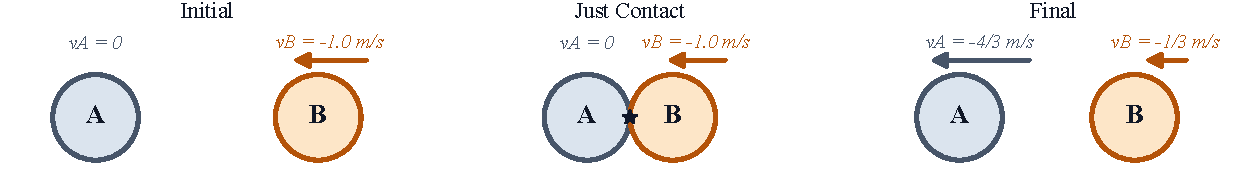
\includegraphics[width=\linewidth]{headon_unequal_mass_spheres_states.pdf}
    \caption{Three-stage model illustration of the unequal-mass head-on collision case. From left to right: initial state, first contact, and final state. Velocity arrows indicate the motion directions of spheres A and B together with the analytical post-impact velocities}
    \label{fig:headon_spheres_massratio_states}
\end{figure}

Figure \ref{fig:headon_spheres_massratio} shows the velocity histories of spheres A and B in the unequal-mass collision. The results indicate that the default shared SDF contact path also aligns pointwise with the analytical piecewise ground truth in this case: the post-impact velocities predicted by both first-order and second-order SDF converge to $-4/3$ m/s and $-1/3$ m/s, respectively, and the corresponding velocity RMSE values for the two spheres are about $2.6\times10^{-7}$. By contrast, the native sphere contact still produces the correct final post-impact velocity, but again exhibits a switching lag on the order of one discrete time step. The resulting velocity RMSE values are $4.22\times10^{-2}$ m/s for sphere A and $2.11\times10^{-2}$ m/s for sphere B. As in the equal-mass case, the discrepancy mainly reflects switching-time bias under the shared time-stepping configuration rather than an error in the final impulse law. This result demonstrates that the current shared SDF contact path reproduces not only equal-mass velocity exchange, but also the correct analytical impulse transfer for the more general unequal-mass head-on elastic impact.

\begin{figure}[!t]
    \centering
    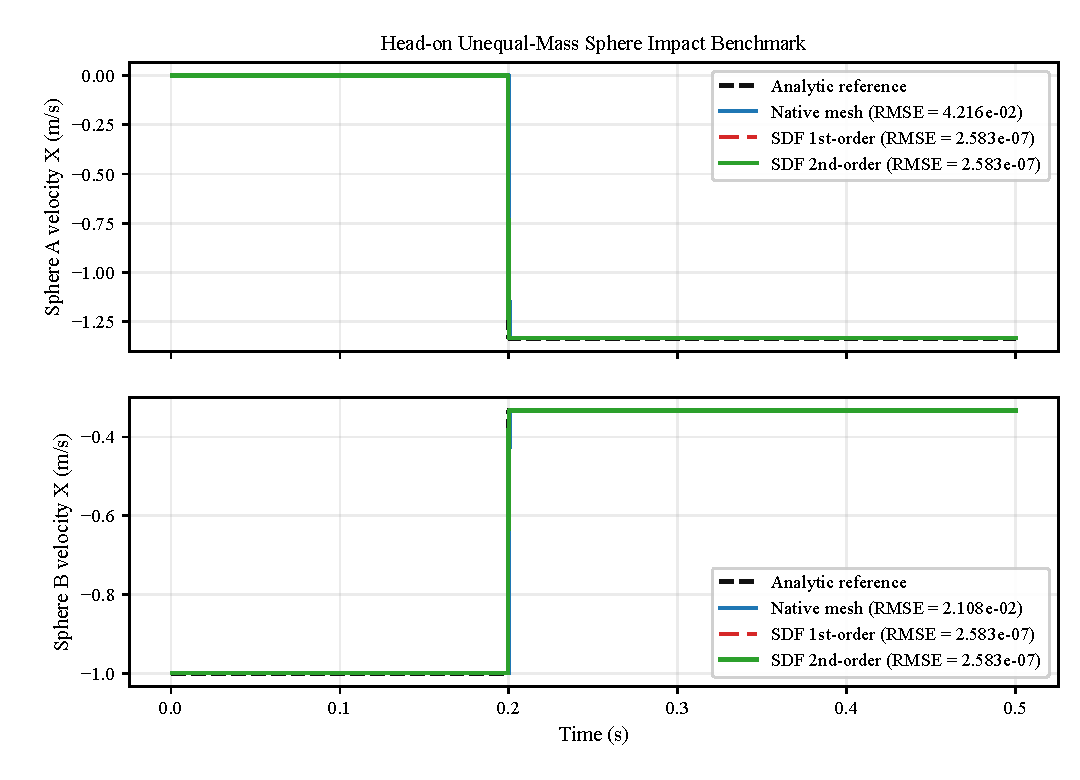
\includegraphics[width=0.94\linewidth]{headon_spheres_massratio_benchmark.pdf}
    \caption{Velocity histories for the unequal-mass elastic head-on impact benchmark, with sphere B twice as heavy as sphere A. Upper: sphere A. Lower: sphere B. The dashed black line denotes the analytical one-dimensional elastic-impact solution. Both SDF variants recover the correct post-impact velocities, while the native mesh again shows a switching lag of one time-step order}
    \label{fig:headon_spheres_massratio}
\end{figure}

\subsection{Continuous-contact capability: analytical roller benchmark (eccentric disk / roller follower)}
To separate the modeling capability for continuous sliding contact itself from possible CAD geometry error, local nonuniform sampling, and contact-switching effects in industrial cam systems, we further construct an analytically verifiable eccentric disk--roller follower benchmark. The driving body is a rigid disk with radius $R=30$ mm and eccentricity $e=6$ mm. The follower is a roller with radius $r=10$ mm constrained to translate along a vertical guide. The driving angular velocity is fixed at $\omega=-2$ rad/s, the simulation horizon is $T=\pi/2$ s, and the integration step size is $\Delta t=0.002$ s. For this geometry, the ideal no-separation motion satisfies
\[
y(t)=e\sin(\omega t)+\sqrt{(R+r)^2-(e\cos(\omega t))^2},
\]
so the numerical solution can be aligned pointwise with the analytical reference trajectory instead of relying on external commercial software output.

This benchmark shares the same LCP + SDF contact backbone as the other cases, but adopts an independent regime configuration better suited to smooth contact with a single dominant normal, with sample-side OBB/BVH broad phase enabled by default. The results are shown in Fig. \ref{fig:eccentric_roller}. Native mesh contact yields the smallest positional error, with position RMSE $3.0\times10^{-6}$ m and velocity RMSE $9.27\times10^{-4}$ m/s, but at a total runtime of $149.4$ s. First-order SDF reduces the runtime to $2.07$ s, with position RMSE $9.0\times10^{-6}$ m and velocity RMSE $6.94\times10^{-4}$ m/s. After introducing second-order curvature feedforward, second-order SDF further reduces the velocity RMSE to $6.88\times10^{-4}$ m/s while keeping nearly the same runtime ($2.23$ s), and limits the maximum velocity error to $1.20\times10^{-2}$ m/s, which is on the same order as the native mesh result.

The significance of this comparison is that it shows the complete \texttt{SlidingPatch} path itself can produce high-quality results with a substantial efficiency advantage in truly smooth and analytically solvable continuous sliding contact. Moreover, within the shared SDF path, second-order curvature feedforward provides a clear incremental accuracy gain over the first-order SDF formulation. In other words, in this regime-matched continuous-contact setting, higher response accuracy does not require a correspondingly large increase in computational cost. This result is complementary to the later Twin Gear benchmark: the present case shows that curvature feedforward is effective and efficient on smooth continuous manifolds, whereas Twin Gear reveals that a structural error floor remains near $C^0$ singular boundaries.

\begin{figure}[!t]
    \centering
    
\includegraphics[width=0.94\linewidth]{eccentric_roller_benchmark.pdf}
    \caption{Analytical benchmark for an eccentric disk--roller follower. The upper, middle, and lower panels show displacement, velocity, and velocity error relative to the analytical reference, respectively. In this smooth continuous-sliding case, the second-order SDF reduces the velocity error while retaining runtime on the same order as the first-order SDF}
    \label{fig:eccentric_roller}
\end{figure}

\subsection{Contact-onset capability: Onset Stress benchmark (Onset Stress B)}
To further distinguish ``manifold-activation error at first contact'' from ``continuous-sliding error after contact has been established,'' we construct a Version B stress test by adding a weak follower return spring--damper to the positive-gap eccentric disk--roller model of Version A. The geometry remains smooth, the target onset time stays the same ($t_{\mathrm{on}}\approx 0.15$ s), and the same analytical reference is retained. The weak preload causes the follower to remain close to the envelope after contact onset instead of detaching in an approximately free-flight manner as in Version A. The model configuration is shown in Fig. \ref{fig:onset_model}.

\begin{figure}[!htbp]
    \centering
    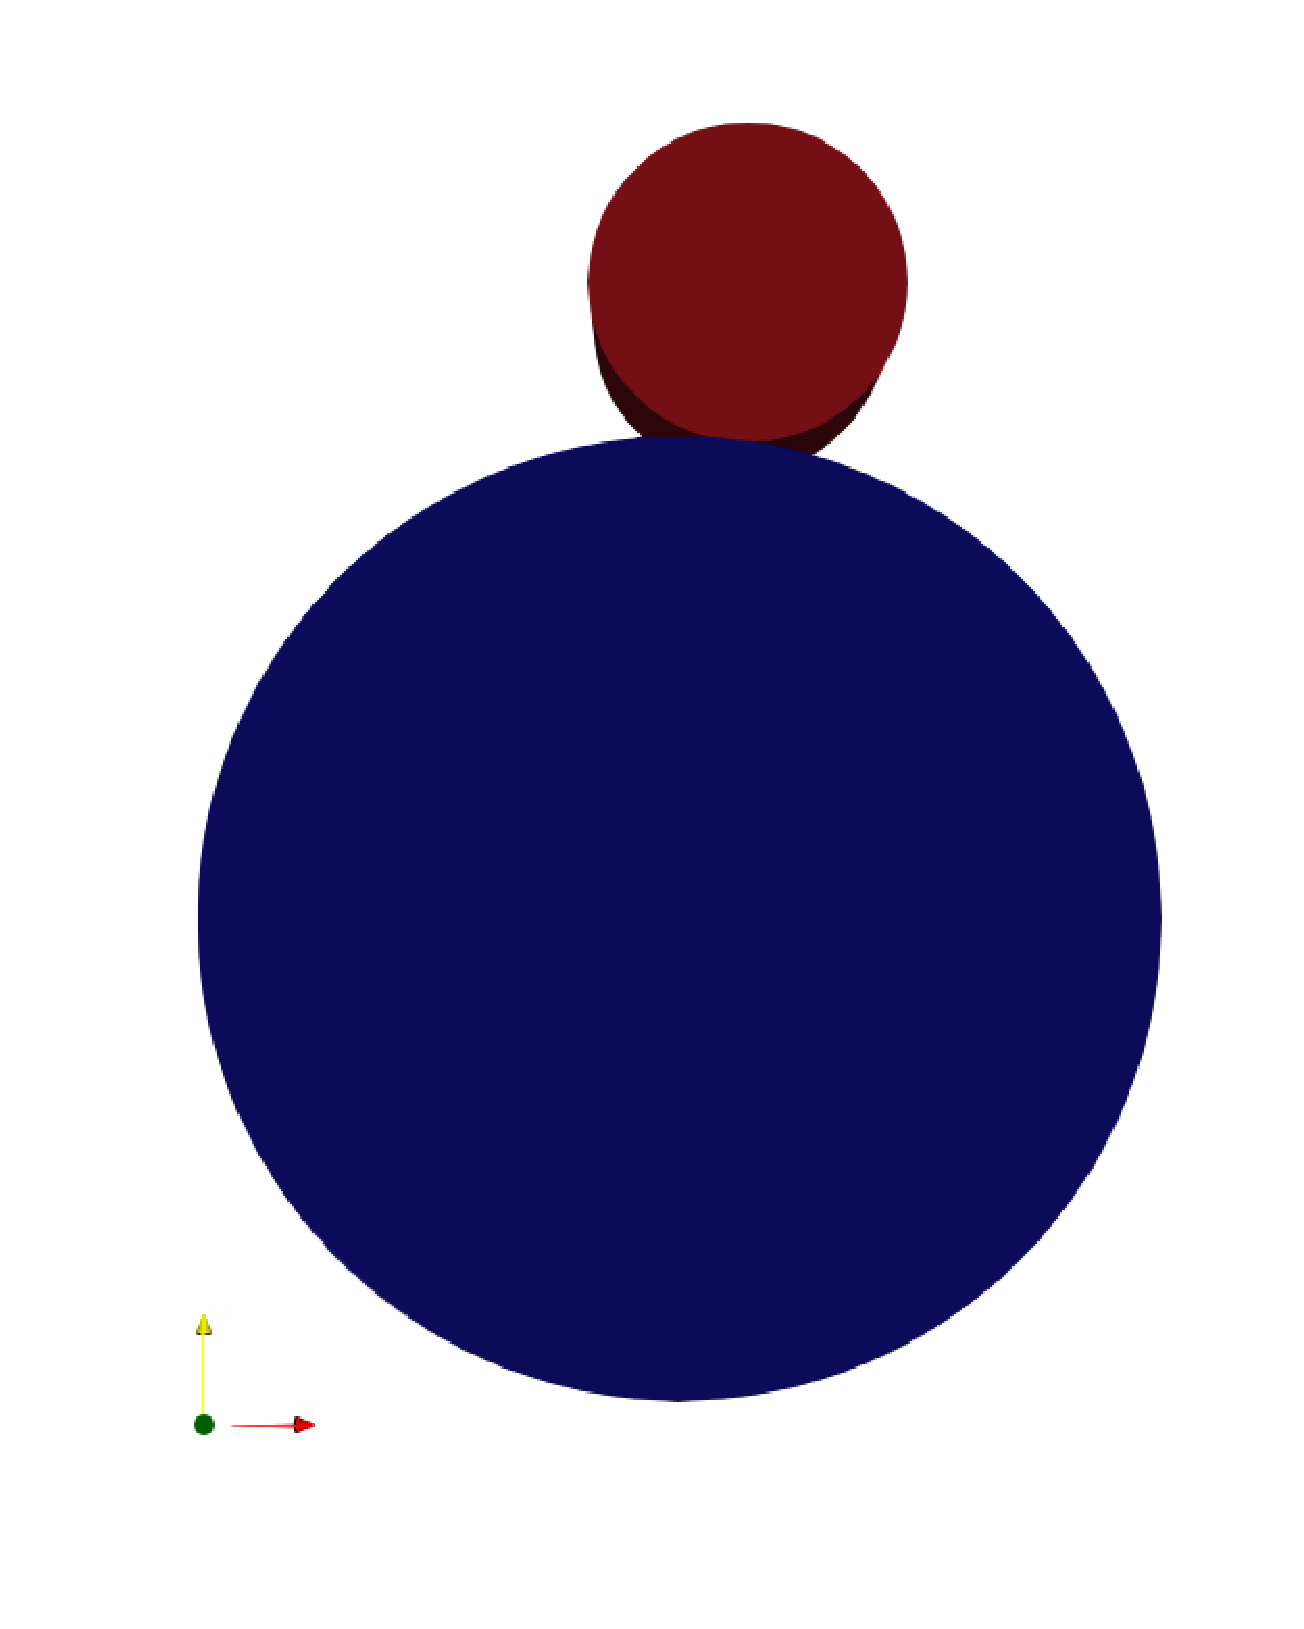
\includegraphics[width=0.54\linewidth]{onset.pdf}
    \caption{Model illustration of the Onset Stress B case. The figure shows the cam--roller system with a weakly preloaded return spring--damper, including the positive-gap initial state and the subsequent sustained-contact stage}
    \label{fig:onset_model}
\end{figure}

In the converged default setting, Version B uses $\Delta t = 0.001$ s, 32 dynamics substeps, an SDF voxel resolution of $100\,\mu$m, and follower return spring--damper parameters $k=670$ N/m and $c=47$ Ns/m, with sample-side OBB/BVH broad phase enabled by default. The results are shown in Fig. \ref{fig:onset_stress_b}. Native mesh contact yields a velocity RMSE of $8.59\times10^{-4}$ m/s and a total runtime of $111.5$ s. First-order SDF achieves a velocity RMSE of $8.43\times10^{-4}$ m/s with a total runtime of $35.4$ s, while second-order SDF further reduces the RMSE to $8.41\times10^{-4}$ m/s with a runtime of $36.4$ s. In other words, on this stress case designed specifically for sustained sliding after onset, both SDF curves already match and slightly exceed native mesh in terms of velocity RMSE after the introduction of continuous-contact-oriented candidate screening, local geometric fitting, and higher temporal resolution, with second-order SDF achieving the best result.

The significance of this result is that the persistent sliding manifold, local geometric fitting, and onset-aware candidate filtering added for continuous sliding do not merely ``appear effective'' in more complex industrial cam benchmarks, but genuinely recover long-term adherence in a controlled stress benchmark with analytically known onset time and an independently assessable sustained-contact phase. Combined with the runtime data, this also shows that the accuracy gain is not purchased by a dramatic increase in cost, but is achieved at a total runtime still far below that of native mesh contact. At the same time, the difference between first-order and second-order results indicates that curvature feedforward still provides an additional, though relatively moderate, incremental gain within this complete continuous-contact modeling stack. Compared with the eccentric benchmark, Version B places more emphasis on the difficulty of maintaining contact after transitioning from a free-gap state into contact; compared with the later Twin Gear benchmark, it avoids $C^0$ singular boundaries and nearest-point branch competition, and therefore provides a cleaner validation of local-geometry-aware modeling in continuous contact.

\begin{figure}[!t]
    \centering
    
\includegraphics[width=0.94\linewidth]{onset_stress_benchmark.pdf}
    \caption{Onset Stress Benchmark Version B. The upper, middle, and lower panels show displacement, velocity, and velocity error relative to the piecewise analytical reference, respectively. In the sustained-sliding phase, both SDF variants match or slightly outperform native mesh in velocity RMSE, with the second-order SDF giving the best result}
    \label{fig:onset_stress_b}
\end{figure}

\clearpage

\subsection{Industrial-scale performance: cam under the base time step}
We now move to the continuous-contact response of an industrial cam--follower system under the base time step. Errors in this benchmark are measured against third-party reference curve data. The current setup uses the \texttt{SlidingPatch} contact representation, a base time step of $\Delta t = 0.005$ s, and an SDF voxel resolution of $4\times 10^{-4}$ m. This corresponds to a relatively fine temporal resolution, under which all three methods track the reference trajectory stably, making it appropriate for comparing error distributions and local peak suppression across different contact representations. The model states are shown in Fig. \ref{fig:cam_model}, where the three views from left to right correspond to the initial state, the instant of first contact, and the final simulation time.

\begin{figure}[!htbp]
    \centering
    \begin{minipage}[t]{0.32\linewidth}
        \centering
        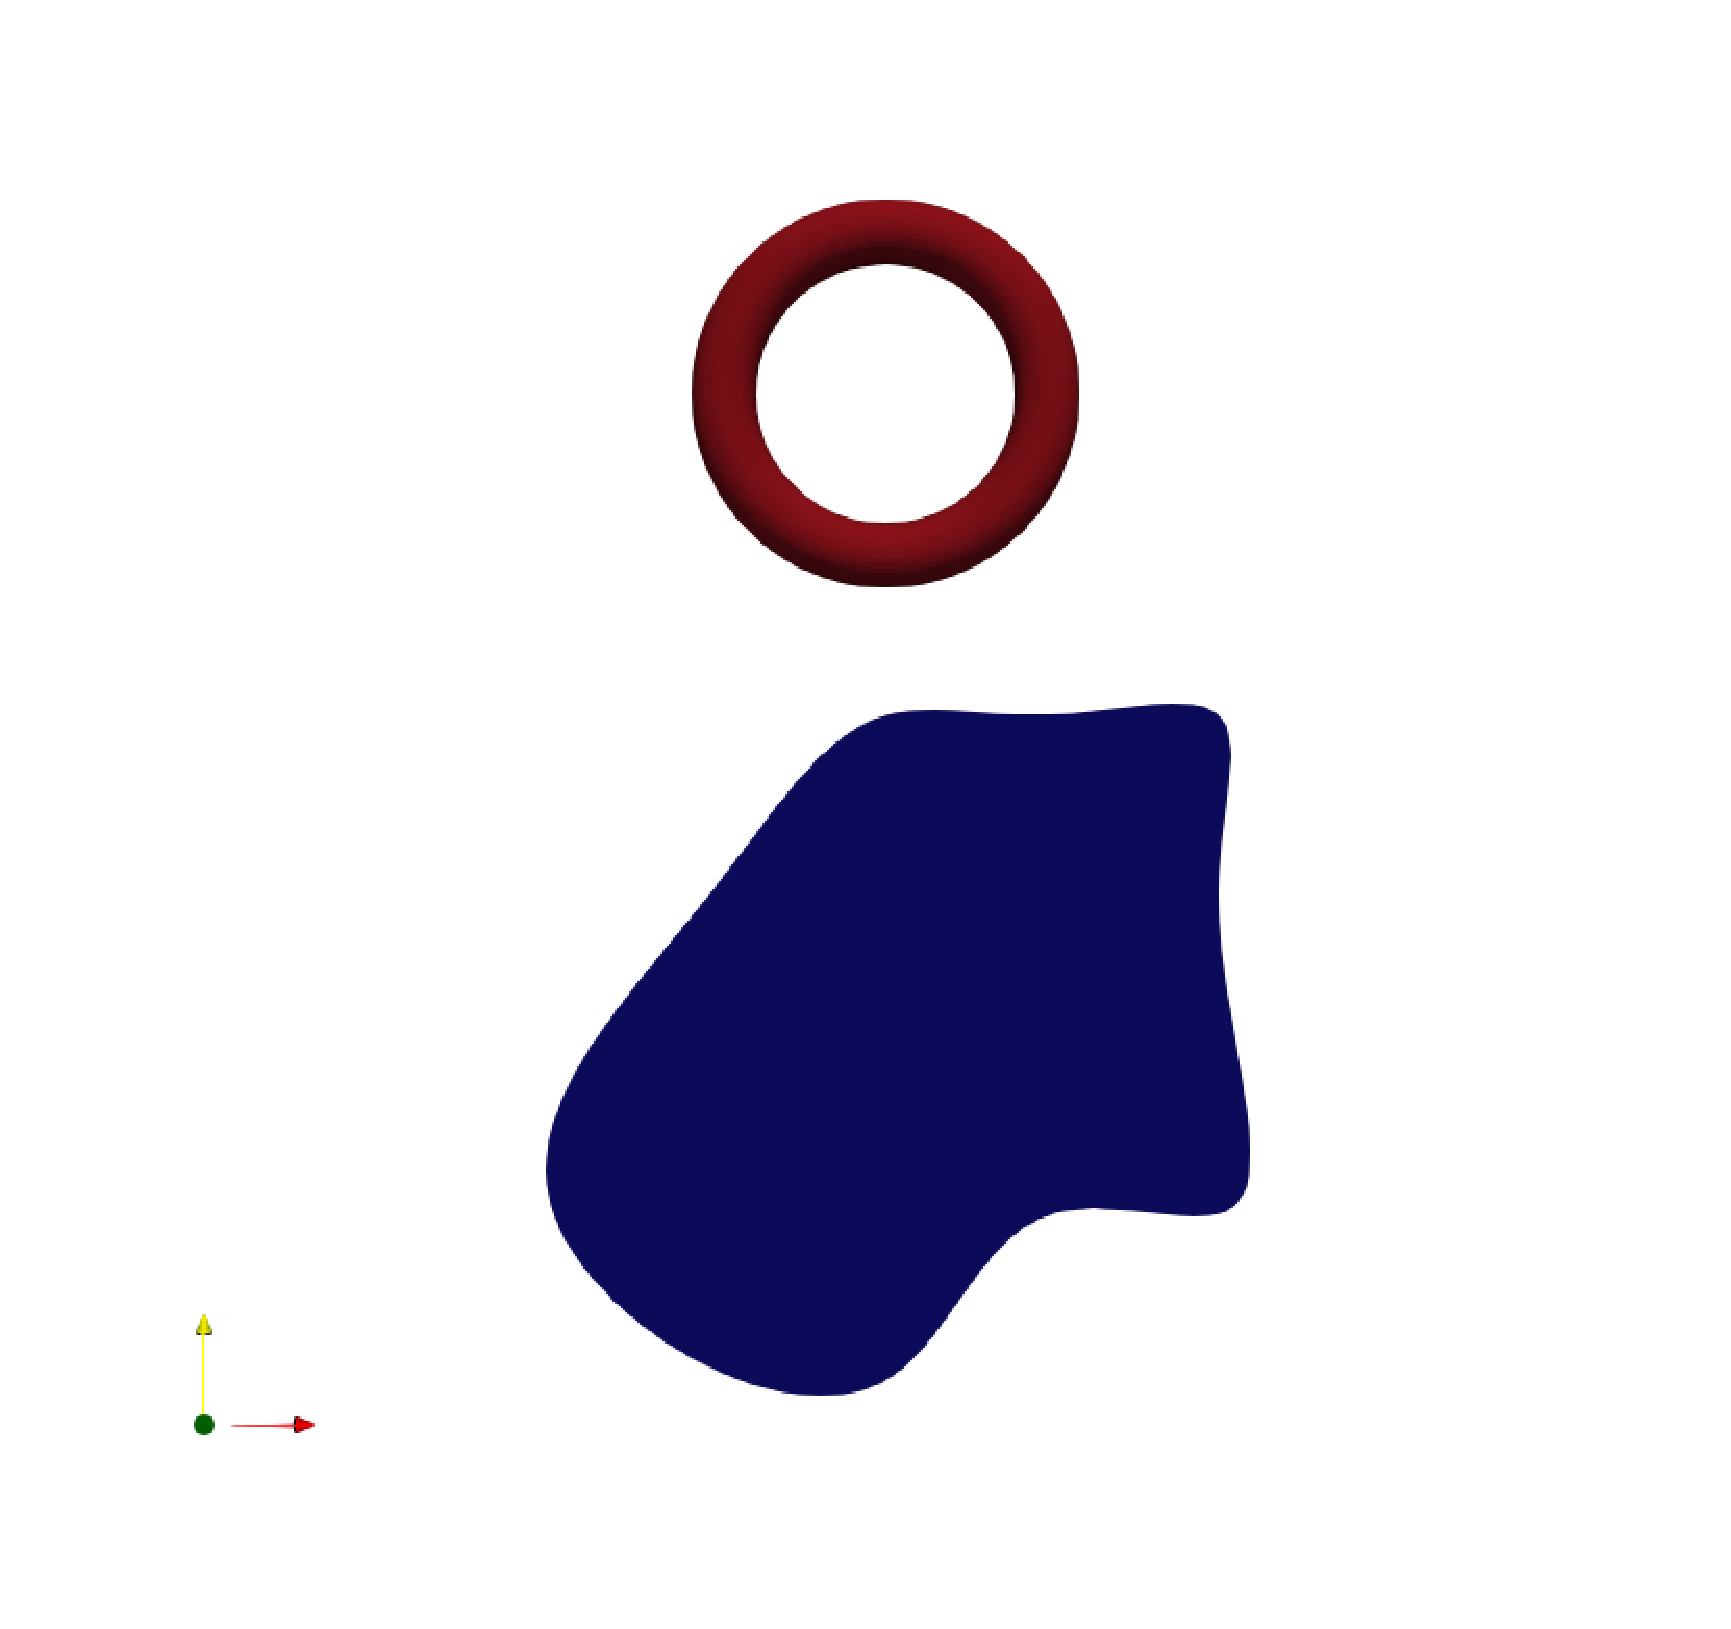
\includegraphics[width=\linewidth]{cam_0.pdf}
    \end{minipage}\hfill
    \begin{minipage}[t]{0.32\linewidth}
        \centering
        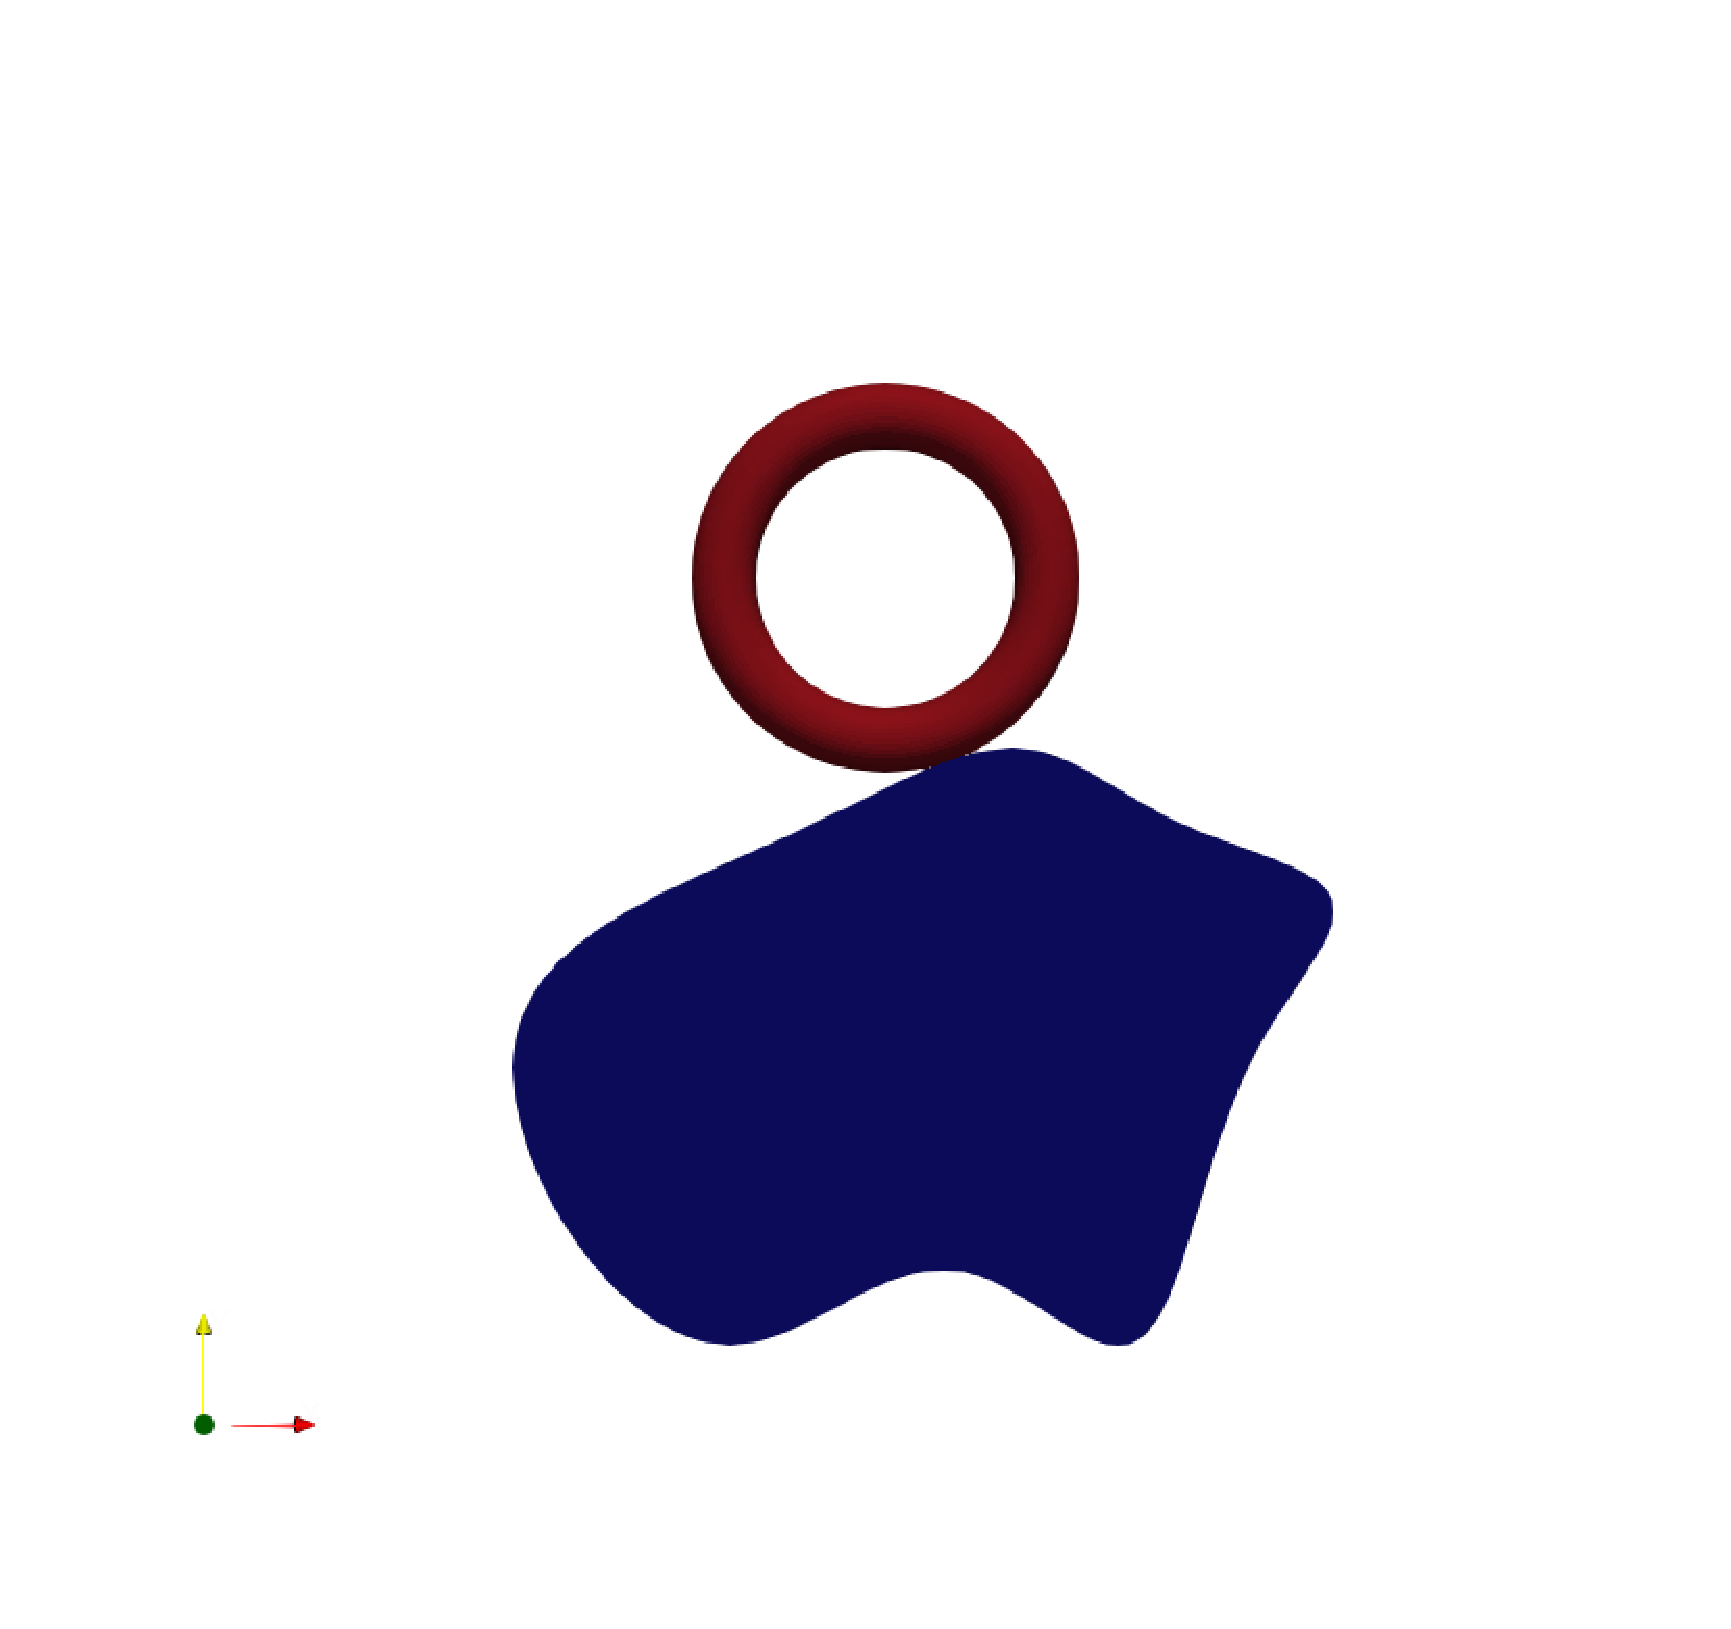
\includegraphics[width=\linewidth]{cam_1.pdf}
    \end{minipage}\hfill
    \begin{minipage}[t]{0.32\linewidth}
        \centering
        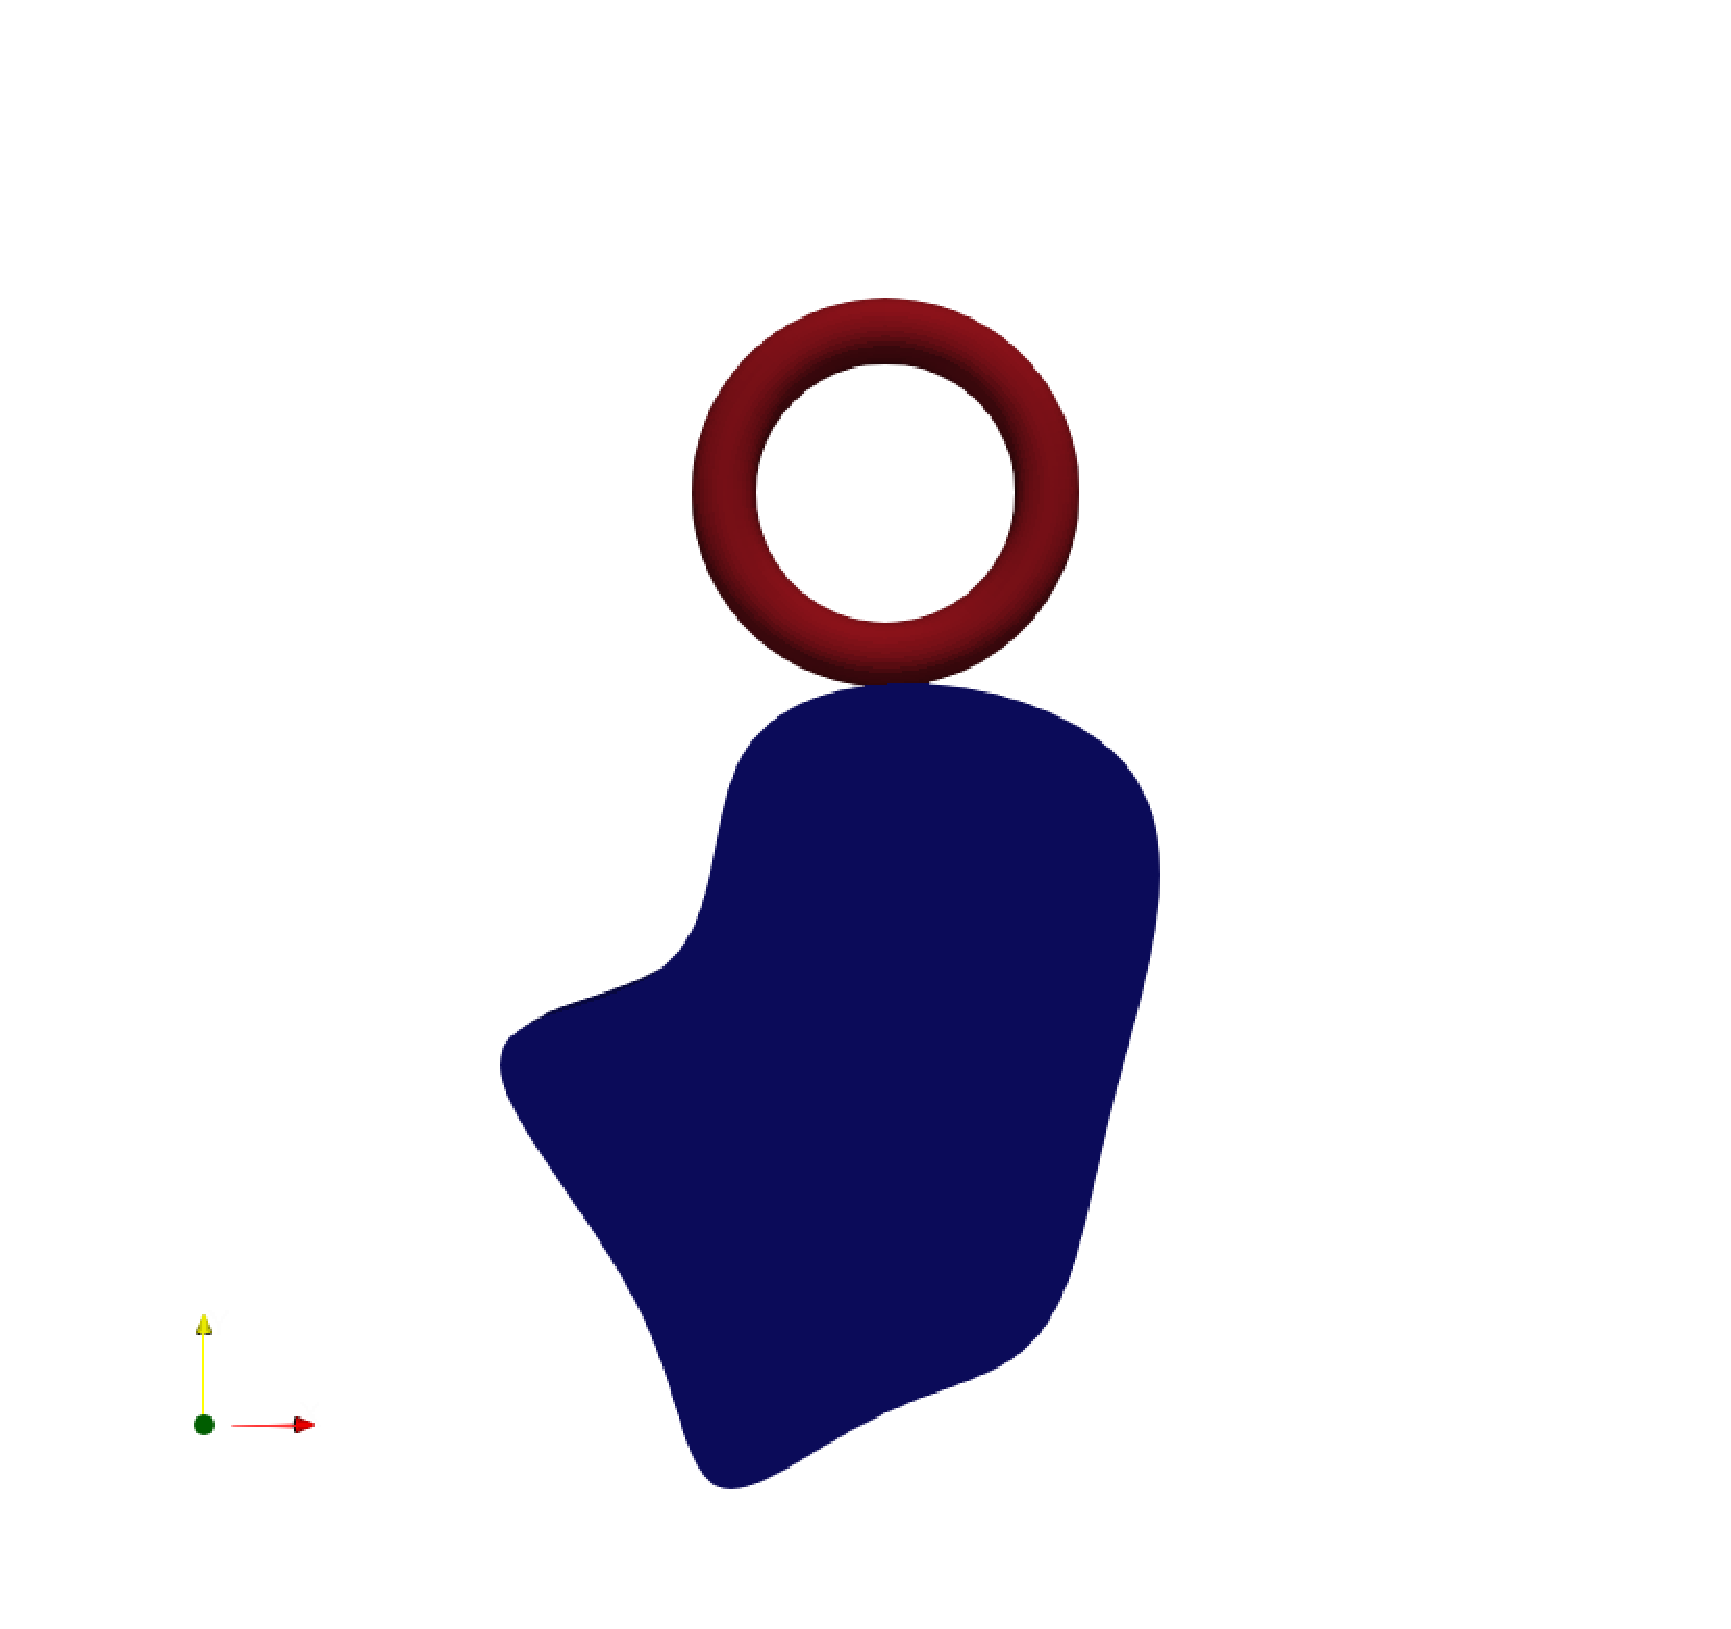
\includegraphics[width=\linewidth]{cam_2.pdf}
    \end{minipage}
    \caption{Model-state illustration of the industrial cam benchmark. From left to right: initial state, first contact, and final simulation time}
    \label{fig:cam_model}
\end{figure}

As shown in Fig. \ref{fig:accuracy}, native mesh, first-order SDF, and second-order SDF all remain stable over the full time window. The velocity RMSE is $3.4347\times 10^{-2}$ m/s for \texttt{Native Mesh}, $3.4209\times 10^{-2}$ m/s for \texttt{SdfFirstOrder}, and $3.1601\times 10^{-2}$ m/s for \texttt{SdfSecondOrder}. This indicates that, at the smaller time step, the full \texttt{SlidingPatch} path already tracks the reference curve stably, while second-order curvature feedforward still provides an additional reduction in global error.

In terms of local peaks, the SDF path also clearly outperforms native mesh. The maximum absolute velocity error of the mesh result is about $5.531\times 10^{-1}$ m/s, whereas the first- and second-order SDF results reduce it to $1.781\times 10^{-1}$ m/s and $1.725\times 10^{-1}$ m/s, respectively. This shows that under a small time step, the benefit of the second-order curvature term is not primarily a dramatic reshaping of the entire trajectory; rather, it is reflected mainly in the further suppression of a small number of locally poor windows. When local Hessian gating is consistent with the manifold-tracking strategy, second-order feedforward can yield a measurable net improvement without compromising stability.

\begin{figure}[!htbp]
    \centering
    
\includegraphics[width=0.94\linewidth]{fig_accuracy.pdf}
    \caption{Velocity response of the industrial cam benchmark at the base time step ($\Delta t = 0.005\text{s}$). All three solutions remain stable. The first-order SDF is comparable to the mesh result in overall RMSE but suppresses peak error more effectively, while the second-order SDF achieves the smallest overall RMSE and peak error}
    \label{fig:accuracy}
\end{figure}

\subsection{Industrial-scale performance: cam under a larger time step}
The time step of the industrial cam benchmark is then increased to $\Delta t = 0.01$ s in order to assess stability and error variation under coarser temporal resolution. Under this setting, all three methods complete the integration stably, but their accuracy levels become clearly separated:
\begin{itemize}
    \item \textbf{Native Mesh:} remains stable, but with the largest velocity error. The velocity RMSE is $5.7619\times 10^{-2}$ m/s and the maximum absolute velocity error is $7.035\times 10^{-1}$ m/s.
    \item \textbf{First-order SDF:} also remains stable and reduces the velocity RMSE to $3.3442\times 10^{-2}$ m/s, indicating that the current continuous-contact representation already supports first-order SDF solving under relatively coarse time stepping.
    \item \textbf{Second-order SDF:} further reduces the velocity RMSE to $2.4831\times 10^{-2}$ m/s while preserving stability, and yields the smallest maximum absolute velocity error of $1.572\times 10^{-1}$ m/s among the three methods.
\end{itemize}

As shown in Fig. \ref{fig:robustness}, both \texttt{SdfFirstOrder} and \texttt{SdfSecondOrder} remain stable at the larger time step and outperform native mesh overall, with second-order curvature feedforward producing the smallest global error and peak error. This indicates that as the temporal resolution becomes coarser, the advantage of the full local-geometry-aware path becomes more pronounced, and the contribution of curvature feedforward within that path also becomes more visible, providing additional accuracy gains and peak suppression. Together with the previous subsection, this suggests a clear time-step dependence of the second-order term: its benefit becomes more fully expressed under coarser time resolution.

\begin{figure}[!htbp]
    \centering
    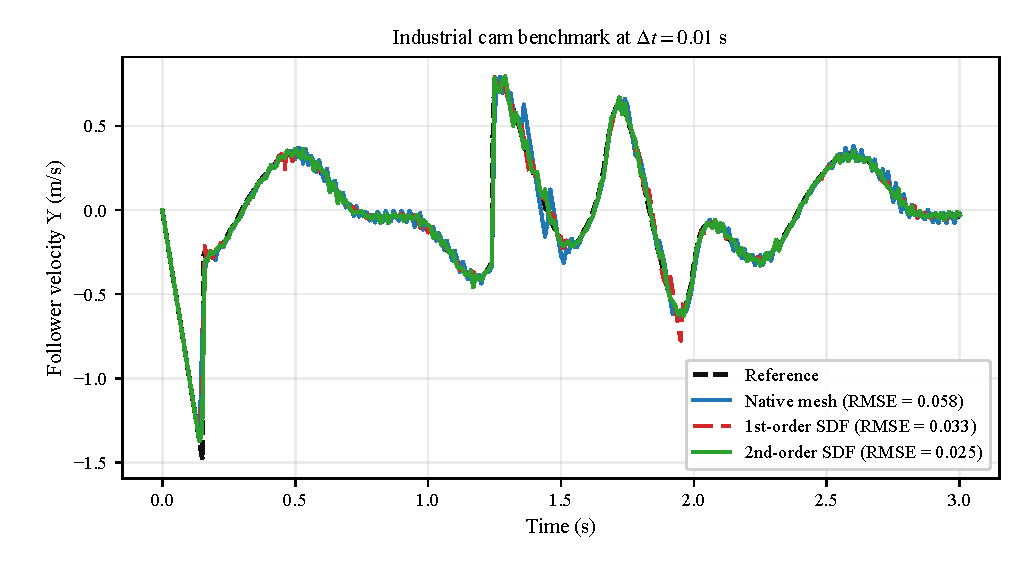
\includegraphics[width=0.94\linewidth]{fig_robustness.pdf}
    \caption{Velocity response of the industrial cam benchmark at the larger time step ($\Delta t = 0.01\text{s}$). Both SDF variants remain stable and outperform native mesh, with the second-order SDF giving the smallest velocity RMSE and peak error}
    \label{fig:robustness}
\end{figure}

\subsection{Remaining limitation: Twin Gear meshing (Twin Gear Benchmark)}
Although second-order Hessian compensation was originally designed for high-curvature contact on smooth manifolds, its performance in complex assemblies containing sharp features ($C^0$ continuity) and small backlash is equally worth separate examination. To evaluate the practical effectiveness of the method at nonsmooth boundaries, we introduce a 1:1 spur-gear meshing validation model (Twin Gear Benchmark), which simulates strongly varying multi-point contact in an extremely confined space. The mean absolute error (MAE) of the follower gear angular velocity is measured uniformly over the full time window $0 \sim 1.0$ s. The overall assembly and the local meshing region are shown in Fig. \ref{fig:twin_gear_model}.

\begin{figure}[!htbp]
    \centering
    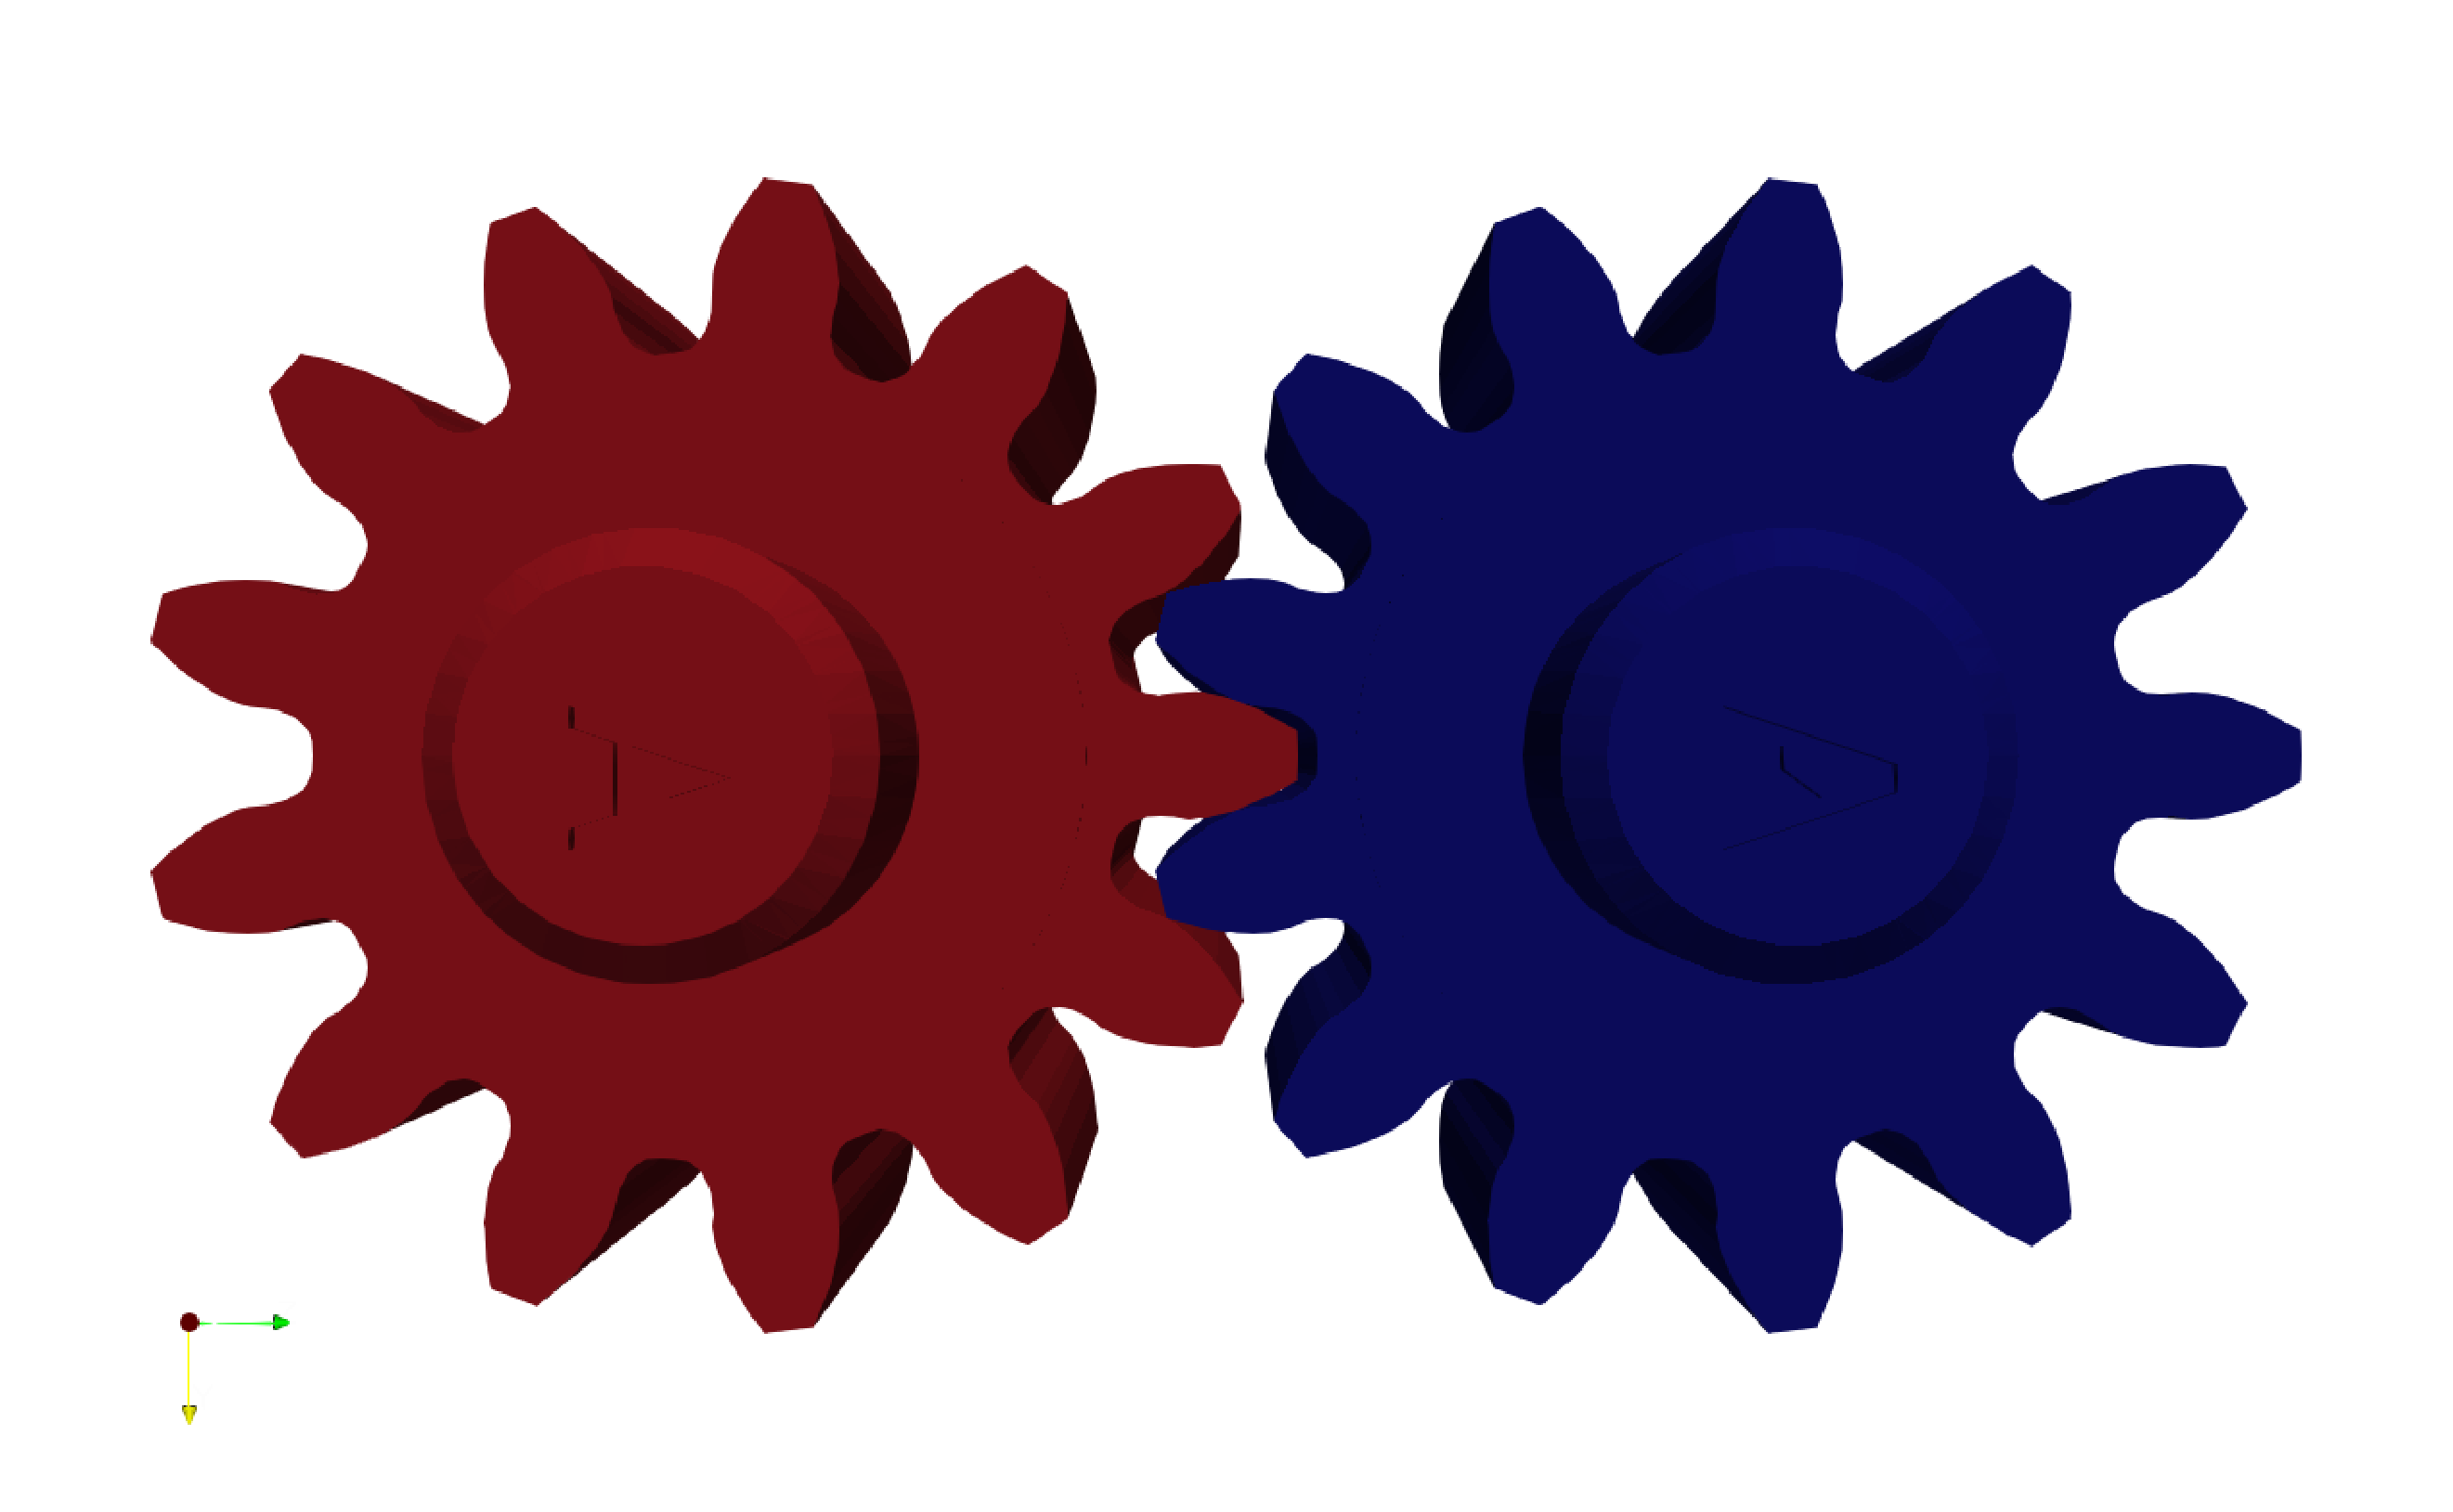
\includegraphics[height=0.35\linewidth]{gear.pdf}\hspace{0.02\linewidth}%
    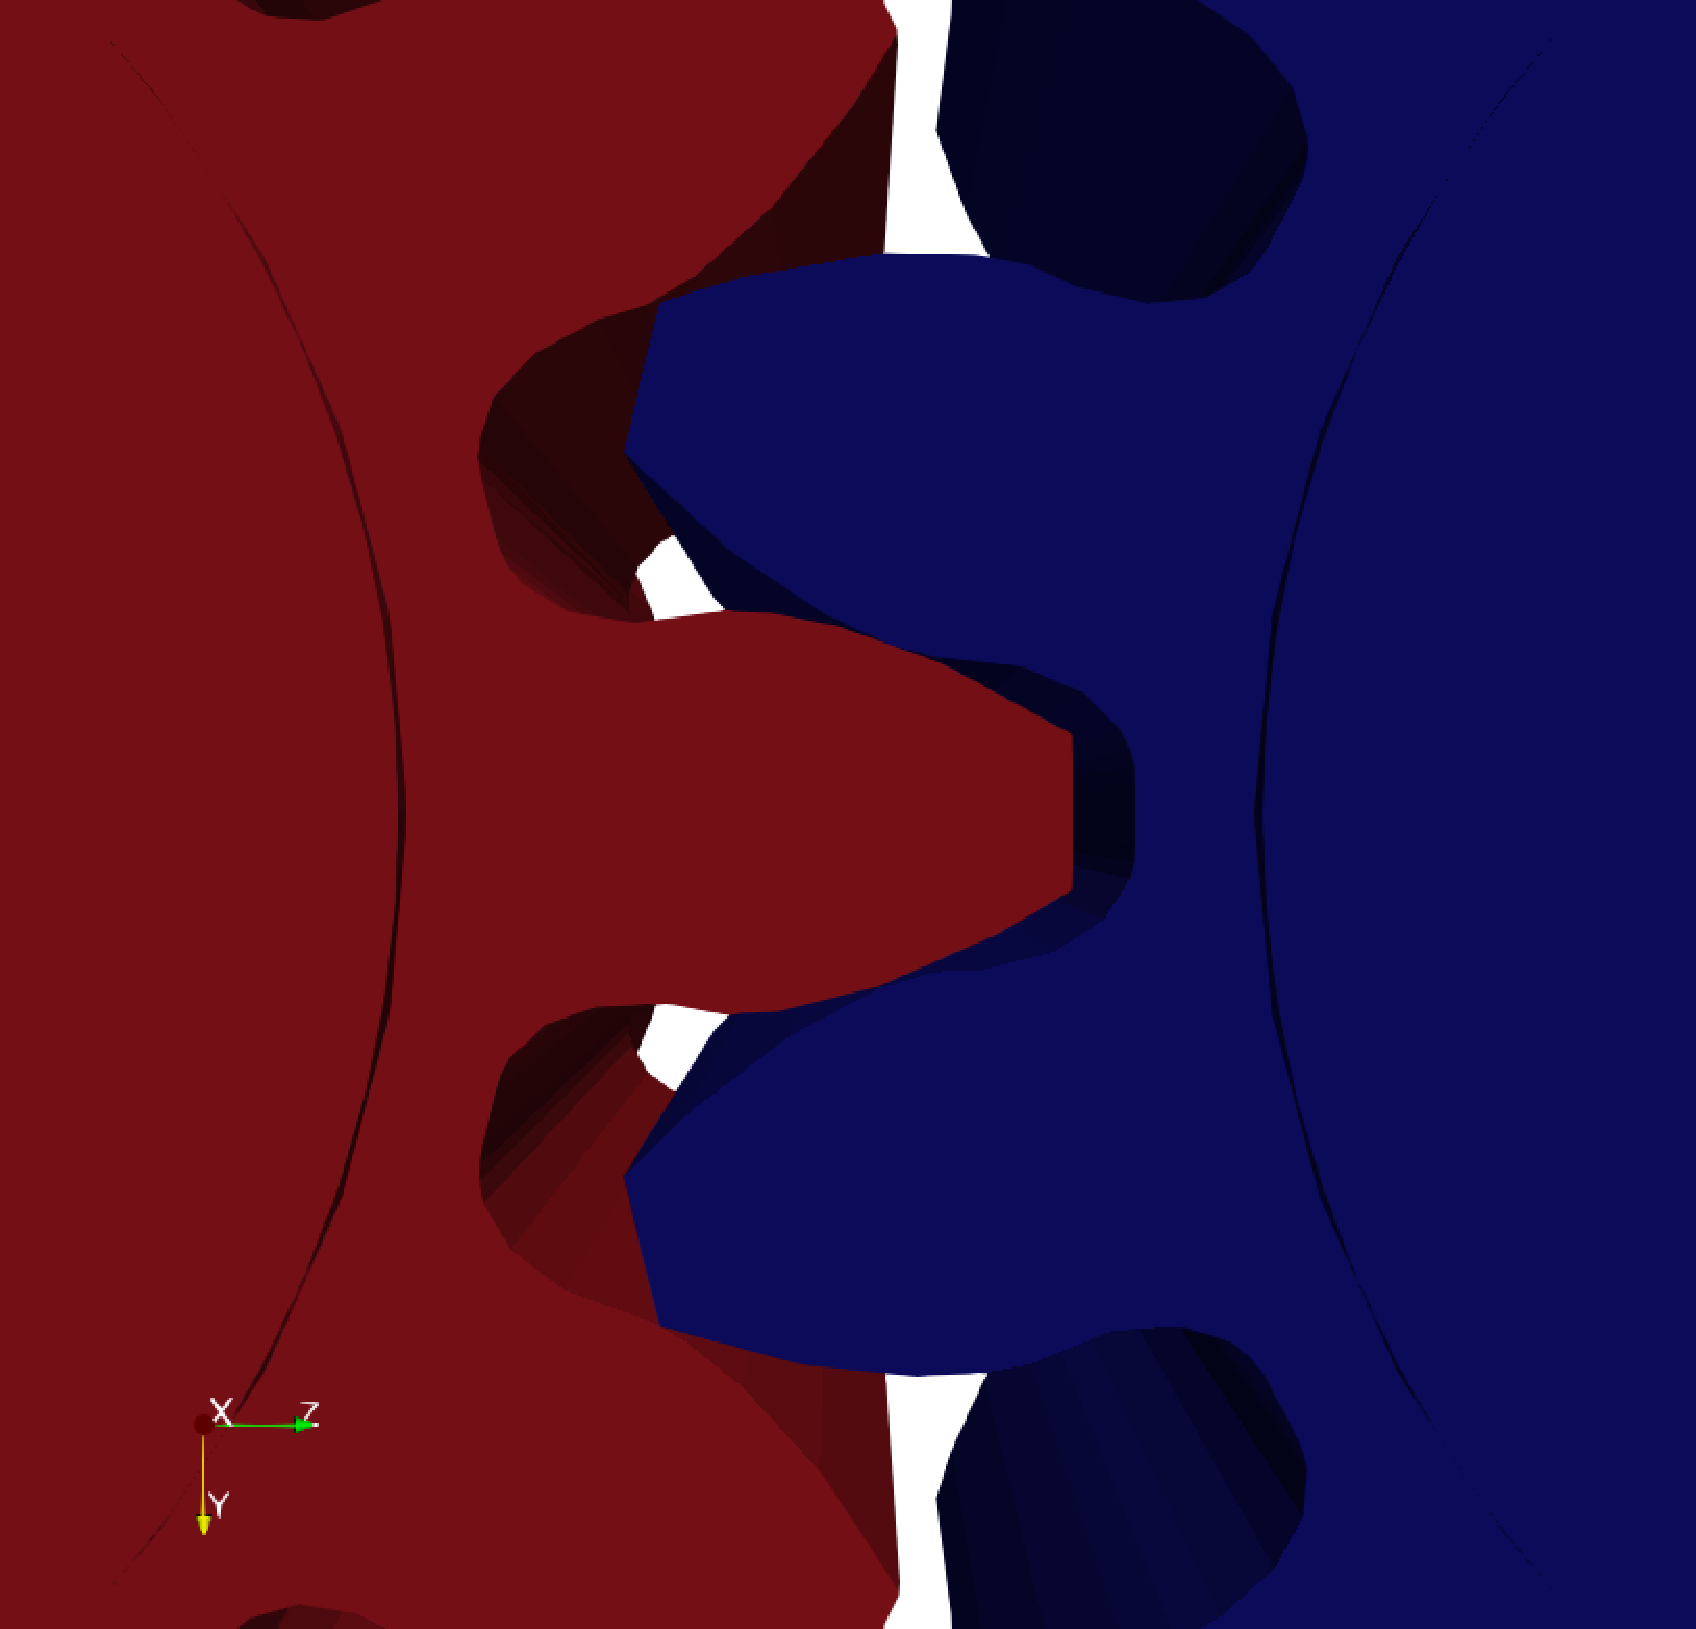
\includegraphics[height=0.35\linewidth]{gear_contact_detail.pdf}
    \caption{Model illustration of the Twin Gear benchmark. The left panel shows the overall 1:1 spur-gear assembly, and the right panel shows the local meshing region near the $C^0$ tooth-boundary transition}
    \label{fig:twin_gear_model}
\end{figure}

Under the current implementation, after introducing patch-level clustering, normal averaging, separating-velocity cutoff, and deepest-sample geometry retention, the second-order gear result no longer exhibits the early-stage degradation in which the overall error was worse than the first-order result. At a high-resolution voxel reconstruction of $20 \mu\text{m}$, the MAE of the commercial industrial baseline (Reference) is $0.0579$ rad/s; the MAE of first-order SDF is $0.0934$ rad/s; and second-order SDF further reduces it to $0.0839$ rad/s. In other words, in the current code state, second-order curvature feedforward is already able to achieve a net improvement over the first-order model in the complex gear-meshing scenario.

This improvement does not imply that the singular-geometry problem has been completely resolved. Figure \ref{fig:gear_error} shows that the second-order model indeed reduces local oscillations in the tooth-transition region and follows the global envelope more closely, but a visible gap still remains relative to the commercial industrial baseline. The reason is that at true topological singularities, such as the junction between tooth tip and tooth flank, the nearest-point branch of the signed distance field switches violently, and the dependence of the second-order curvature term on the local normal manifold remains disturbed by the nonsmooth boundary. The current patch-level manifold reduction and contact-screening strategy substantially suppress this singular feedback, but it is still insufficient to remove all residual pulses within a point-contact differential framework.

Accordingly, the current gear benchmark supports the following conclusion: \textbf{after the introduction of appropriate contact-patch reduction and geometric screening, the SDF contact path with curvature feedforward can still achieve a measurable net improvement over the first-order model even near $C^0$ singular boundaries; however, the attainable accuracy remains limited by the sensitivity of point-contact Taylor expansion to nonsmooth nearest-point branch switching.} This result shows that second-order curvature feedforward has practical value in complex assemblies, while also indicating that further progress toward industrial-grade accuracy will likely require moving beyond local point-differential formulations toward higher-dimensional integral SDF or volumetric contact representations.

\begin{figure}[!t]
    \centering
    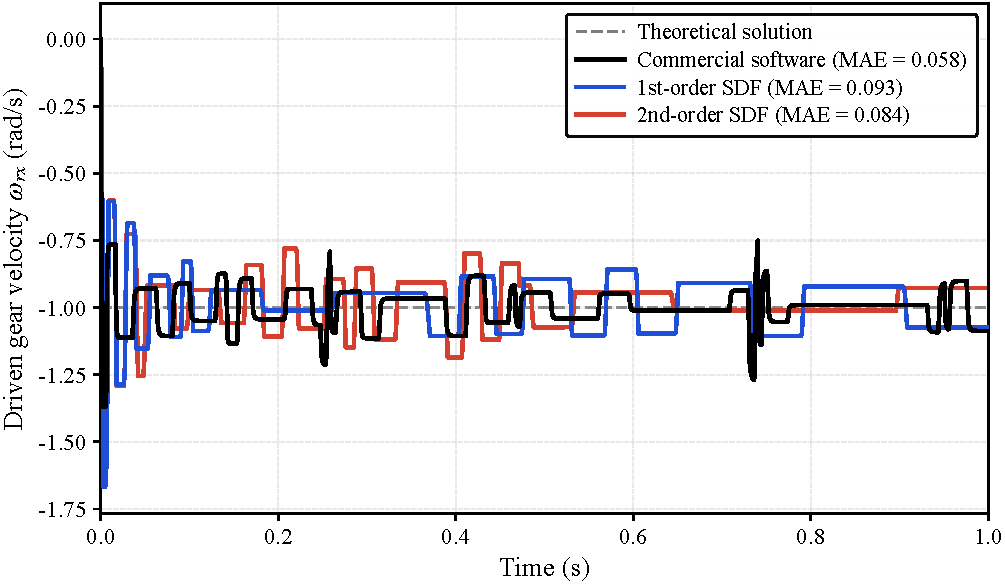
\includegraphics[width=0.94\linewidth]{gear_error.pdf}
    \caption{Transient follower-gear angular velocity response and error analysis for the Twin Gear benchmark under different curvature strategies. In the current implementation, second-order SDF improves upon first-order SDF in full-window MAE and suppresses local oscillations in the tooth-transition region, but visible residual error remains relative to the commercial industrial baseline}
    \label{fig:gear_error}
\end{figure}

\subsection{Engineering efficiency: runtime summary}
After analyzing correctness, accuracy, and limitations, we finally summarize the runtime performance of the proposed method from the standpoint of engineering deployment. Unless otherwise stated, sample-side OBB/BVH broad phase is enabled by default in the three representative continuous-sliding benchmarks considered here, namely the industrial cam, the eccentric disk--roller analytical benchmark, and the Onset Stress Benchmark, so as to reduce candidate-query cost during active-set construction. For Twin Gear, it remains disabled by default and is used only in offline comparisons to verify losslessness and benefit boundaries. This setting reflects a basic principle of the present work: hierarchical broad phase must also be matched to the preset regime and the associated local manifold shape, rather than being uniformly forced on all benchmarks.

For practical deployment in engineering-scale complex assembly simulation, the additional algorithmic overhead is critical because both explicit and implicit multibody stepping are subject to strict runtime constraints. In the current implementation, native mesh contact still relies on an explicit mesh-geometry contact chain, whereas the SDF path reuses the same LCP solution backbone and adds sample-side OBB/BVH broad phase only in continuous-sliding benchmarks. Tables \ref{tab:runtime_overview} and \ref{tab:error_overview} therefore report the formal runtime and main error metrics for three representative continuous-contact benchmarks.

These data show that the extra cost of second-order curvature feedforward does not push the SDF path back into the runtime range of native mesh contact. On the contrary, in the current implementation state, \texttt{SdfSecondOrder} remains on the same order of computational cost as \texttt{SdfFirstOrder} for the industrial cam, eccentric disk--roller, and Onset Stress benchmarks, while delivering consistent net gains in accuracy. For these representative continuous-contact benchmarks, the evidence therefore supports the central claim of this paper: under regime-matched local representations, improved contact-response accuracy can be obtained while keeping computational cost low. The present local-geometry-aware modeling strategy is therefore not simply a matter of ``more expensive contact solving,'' but a way of making efficiency and accuracy coexist through matched local manifold representations and hierarchical candidate detection.

\begin{table}[htbp]
    \centering
    \caption{Total runtime comparison for representative continuous-contact benchmarks}
    \label{tab:runtime_overview}
    \resizebox{\columnwidth}{!}{
    \begin{tabular}{lccc}
        \toprule
        \textbf{Benchmark} & \textbf{Native Mesh} & \textbf{SDF 1st-order} & \textbf{SDF 2nd-order} \\
        \midrule
        Industrial cam ($\Delta t=0.01$ s, $T=3.0$ s) & $135.9$ s & $15.0$ s & $16.0$ s \\
        Eccentric disk--roller ($\Delta t=0.002$ s, $T=\pi/2$ s) & $149.4$ s & $2.07$ s & $2.23$ s \\
        Onset Stress B ($\Delta t=0.001$ s) & $111.5$ s & $35.4$ s & $36.4$ s \\
        \bottomrule
    \end{tabular}
    }
\end{table}

\begin{table}[htbp]
    \centering
    \caption{Main error metrics for representative continuous-contact benchmarks}
    \label{tab:error_overview}
    \resizebox{\columnwidth}{!}{
    \begin{tabular}{lccc}
        \toprule
        \textbf{Benchmark} & \textbf{Native Mesh} & \textbf{SDF 1st-order} & \textbf{SDF 2nd-order} \\
        \midrule
        Industrial cam (velocity RMSE) & $0.0576$ & $0.0334$ & $0.0248$ \\
        Eccentric disk--roller (velocity RMSE) & $9.27\times10^{-4}$ & $6.94\times10^{-4}$ & $6.88\times10^{-4}$ \\
        Onset Stress B (velocity RMSE) & $8.59\times10^{-4}$ & $8.43\times10^{-4}$ & $8.41\times10^{-4}$ \\
        \bottomrule
    \end{tabular}
    }
\end{table}
